



\section{RoPE Effect on Outlier Distribution}\label{sec:outlier_analy}

Let $\mathbf{Q}$, $\mathbf{K}$, and $\mathbf{V}$ denote the query, key, and value matrices, respectively, each belonging to $\mathbb{R}^{N \times D}$, where $N$ represents the sequence length and $D$ denotes the feature dimension.

In DiT-based video generation models, 3D RoPE is widely adopted to capture complex spatiotemporal dependencies. Theoretically, the feature dimension $D$ of the $\mathbf{Q}$ and $\mathbf{K}$ matrices is partitioned into \textbf{three distinct segments}---$D_{f}$, $D_{h}$, and $D_{w}$---corresponding to the temporal (frame), height, and width dimensions, respectively, such that $D=D_{f}+D_{h}+D_{w}$.

The 3D RoPE rotary matrix $\mathbf{M} \in \mathbb{R}^{D \times D}$ is a block-diagonal matrix 
composed of $D/2$ fundamental rotation blocks $\mathbf{M}_i \in \mathrm{SO}(2)$. 
This matrix is partitioned into three sub-matrices—$\mathbf{M}^f$, $\mathbf{M}^h$, and 
$\mathbf{M}^w$—each responsible for encoding temporal, height, and width information 
within their respective dimensional segments.




\paragraph{\textbf{Implementation.}} 
Due to the inherent sparsity of the rotary matrix $\mathbf{M}$, the computation of RoPE substitutes the standard matrix multiplication with a more efficient element-wise operation.

\paragraph{\textbf{Outlier Metric.}} 
To analyze the distribution of outliers that predominantly affect quantization precision, we introduce the \textit{incoherence} metric $\Psi(\mathbf{X})$, which captures the maximum deviation within each channel. For a given matrix $\mathbf{X} \in \{\mathbf{Q}, \mathbf{K}\}$, we first compute the sequence-wise mean vector $\mathbb{E}[\mathbf{X}] \in \mathbb{R}^{1 \times D}$:
\begin{equation}
    \mathbb{E}[\mathbf{X}] = \frac{1}{N} \sum_{i=1}^{N} \mathbf{X}_{i,:},
\end{equation}
where $\mathbf{X}_{i,:}$ denotes the $i$-th row of $\mathbf{X}$. The incoherence $\Psi(\mathbf{X}) \in \mathbb{R}^{1 \times D}$ is then defined as:
\begin{equation}
    \Psi(\mathbf{X}) = \max_{i \in \{1,\dots,N\}} \left| \mathbf{X}_{i,:} - \mathbb{E}[\mathbf{X}] \right|,
\end{equation}
where the absolute value and maximum operations are applied element-wise. This metric provides a channel-level statistical profile, reflecting the outlier concentration within $\mathbf{Q}$ and $\mathbf{K}$ that poses challenges for fixed-point quantization.


\subsection{Data Distribution of $\mathbf{Q}$ and $\mathbf{K}$}

\begin{figure*}[t]
  \centering
  \begin{subfigure}{0.48\linewidth}
    \centering
    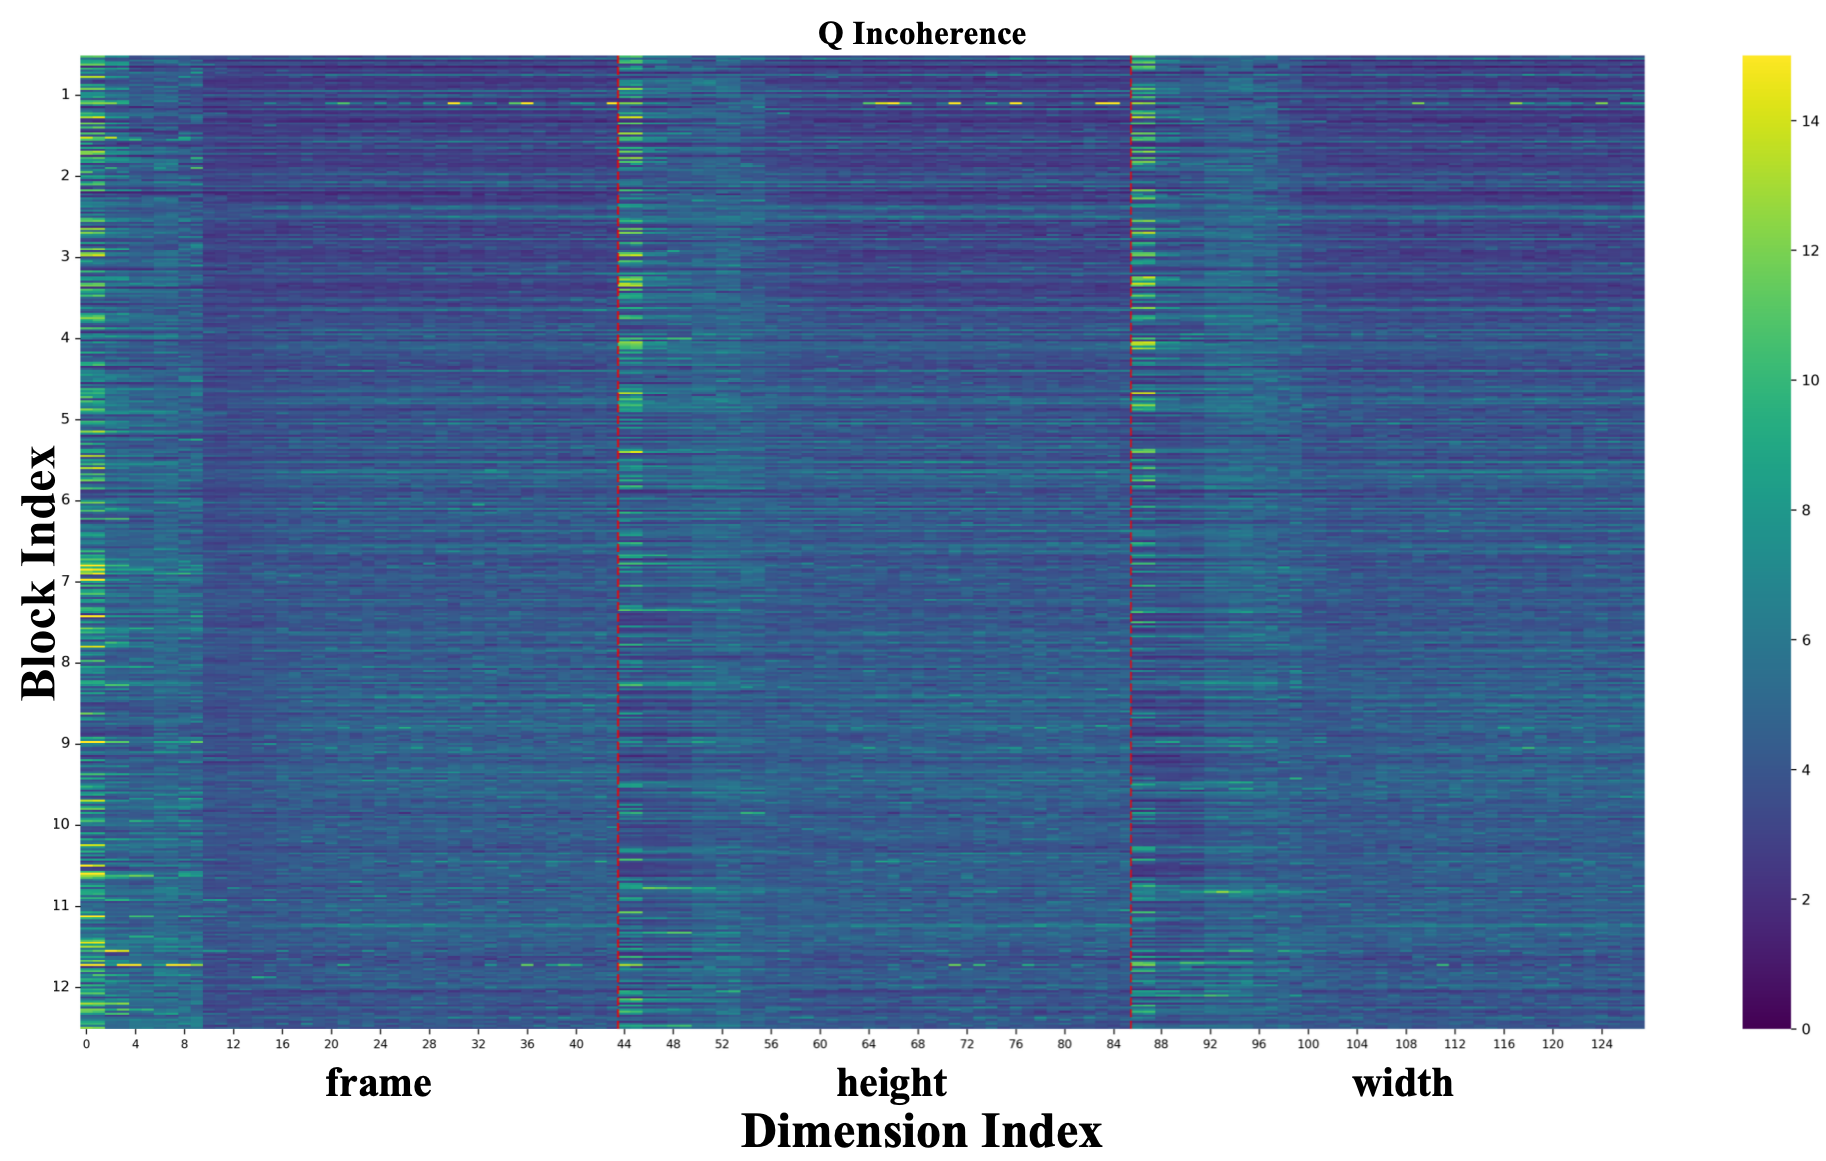
\includegraphics[width=\textwidth]{eccv2026/samll_2/q1.png}
    \caption{$\mathbf{Q}$ Incoherence}
  \end{subfigure}
  \hfill
  \begin{subfigure}{0.48\linewidth}
    \centering
    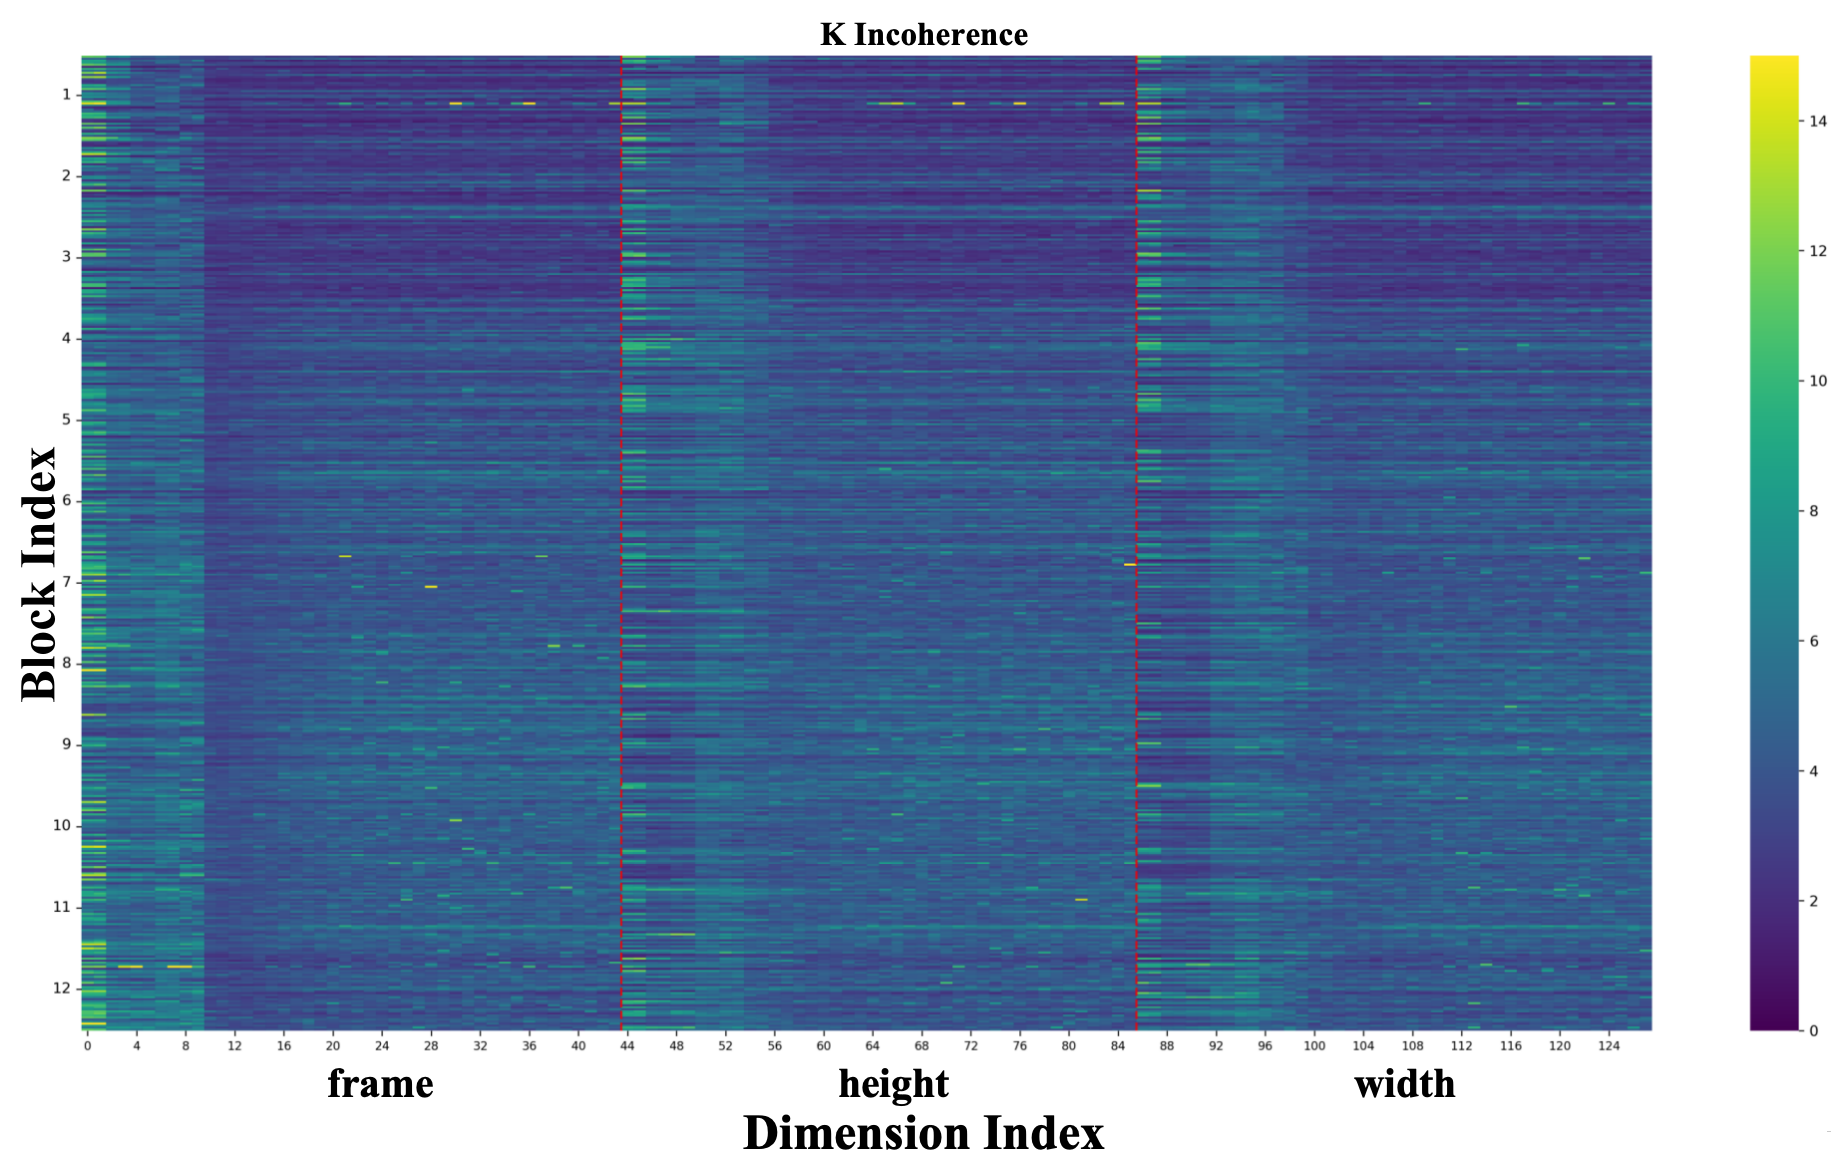
\includegraphics[width=\textwidth]{eccv2026/samll_2/k1.png}
    \caption{$\mathbf{K}$ Incoherence}
  \end{subfigure}

  \vspace{0.8em}

  \caption{\textbf{Channel-wise incoherence profiles of $\mathbf{Q}$ and $\mathbf{K}$ for Wan2.2.} Incoherence is partitioned into three regions corresponding to the 3D RoPE spatiotemporal segments. We observe strong distributional symmetry between $\mathbf{Q}$ and $\mathbf{K}$, and structured sparsity within each segment.}
  \label{fig:incoherent}
\end{figure*}



By evaluating the incoherence $\Psi(\mathbf{X})$ for $\mathbf{X} \in \{\mathbf{Q}, \mathbf{K}\}$, as shown in Fig.~\ref{fig:incoherent}, we identify two key patterns in the outlier distribution:

\paragraph{\textbf{Spatiotemporal Segmental Incoherence.}} 
Outliers are strictly partitioned into three specific segments---frame, height, and width---matching the channel segments defined by the 3D RoPE. Within these segments, we observe that one half of the dimensions typically contains the vast majority of the incoherence, while the remaining half remains relatively smooth.

\paragraph{\textbf{Cross-Matrix Symmetry.}} 
We find that the outlier distribution patterns of $\mathbf{Q}$ and $\mathbf{K}$ exhibit high symmetry. Specifically, channels at identical indices in $\mathbf{Q}$ and $\mathbf{K}$ generally possess nearly equivalent incoherence magnitudes.

\paragraph{\textbf{Theoretical Interpretation.}}
The segmented outlier structure is consistent with 3D RoPE frequency assignment: low-frequency channel pairs accumulate larger angular spread over long sequences and thus higher variance, while high-frequency pairs remain comparatively smooth. Because $\mathbf{Q}$ and $\mathbf{K}$ share RoPE parameters and are projected from the same hidden states, their channel-wise outlier profiles remain symmetric.







\section{Method}
We focus on attention modules in DiT-based video generation models equipped with 3D RoPE. 
We consider queries ($\mathbf{Q}$), keys ($\mathbf{K}$), and values ($\mathbf{V}$), which are equipped with biases shared across all tokens. To address this, we first perform smoothing on $\mathbf{Q}$, $\mathbf{K}$, and $\mathbf{V}$. 

Furthermore, we observe that $\mathbf{Q}$ and $\mathbf{K}$ exhibit specific distributional patterns of outliers. Based on these patterns, we apply a specially designed rotation for the Query and Key matrices to redistribute and equalize these outliers, thereby improving quantization robustness.

\subsection{Rotation for Query and Key}

\paragraph{\textbf{Outlier Equalization via Orthogonal Rotation.}} 
Motivated by these observations, we introduce an orthogonal rotation matrix $\mathbf{R} \in \mathbb{R}^{D \times D}$ to equalize the outlier distribution. We define $\mathbf{R}$ as a block-diagonal matrix:
\begin{equation}
    \mathbf{R} = \mathrm{diag}\left( \{\mathbf{R}_i\}_{i=1}^{D/2} \right),
\end{equation}
where each $\mathbf{R}_i \in \mathrm{O}(2)$ is a $2 \times 2$ orthogonal matrix. When the rotation matrix $\mathbf{R}$ is non-trainable, we initialize the $2 \times 2$ orthogonal blocks $\mathbf{R}_i$ with a $2 \times 2$ Hadamard matrix, defined as:
\begin{equation}
\label{eq:H_2}
\mathbf{H}_{2} = \frac{1}{\sqrt{2}}
\begin{bmatrix}
 1 &  1 \\
 1 & -1
\end{bmatrix}.
\end{equation}



\subsubsection{Mathematical Analysis on the Necessity of Orthogonality}
\label{sssec:orthogonal_property}

To maintain computational equivalence, when a transformation matrix $\mathbf{R}$ is applied to $\mathbf{Q}$, the matrix $\mathbf{K}$ must be transformed by $\mathbf{R}^{-\top}$:
\begin{equation}
    \mathbf{Q}\mathbf{K}^{\top}
    =
    (\mathbf{Q}\mathbf{R})(\mathbf{K}\mathbf{R}^{-\top})^{\top}.
\end{equation}
This equality holds for any invertible $\mathbf{R}$ in full precision. However, under low-bit quantization, the transformation not only changes the coordinate system, but also directly affects the numerical ranges and outlier distributions of the transformed $\mathbf{Q}$ and $\mathbf{K}$. Since $\mathbf{Q}$ and $\mathbf{K}$ usually exhibit symmetric and comparable outlier patterns after RoPE, the transformation should preserve their balance rather than suppressing outliers in one matrix while amplifying them in the other.

Let $\mathbf{R}=\mathbf{U}\mathbf{\Sigma}\mathbf{L}^{\top}$ be the SVD of $\mathbf{R}$, where $\mathbf{U},\mathbf{L}\in\mathbb{O}(D)$ and $\mathbf{\Sigma}=\mathrm{diag}(\sigma_1,\ldots,\sigma_D)$. The corresponding transformation on $\mathbf{K}$ is
\begin{equation}
    \mathbf{R}^{-\top}
    =
    ((\mathbf{U}\mathbf{\Sigma}\mathbf{L}^{\top})^{-1})^{\top}
    =
    \mathbf{U}\mathbf{\Sigma}^{-1}\mathbf{L}^{\top}.
\end{equation}
Therefore, the singular values applied to $\mathbf{K}$ are $\{1/\sigma_i\}_{i=1}^{D}$. If $\sigma_i<1$, the $i$-th principal direction of $\mathbf{Q}$ is compressed, but the corresponding direction of $\mathbf{K}$ is amplified by $1/\sigma_i>1$. Conversely, if $\sigma_i>1$, the outliers in $\mathbf{Q}$ are amplified while those in $\mathbf{K}$ are suppressed. In both cases, anisotropic scaling introduces an asymmetric range change between $\mathbf{Q}$ and $\mathbf{K}$, which can enlarge the quantization error of either matrix.

To avoid this cross-matrix amplification and preserve balanced quantization difficulty, the transformation should impose the same singular scaling on both branches. This requires $\mathbf{\Sigma}=\mathbf{\Sigma}^{-1}$, i.e., $\sigma_i=1$ for all $i$. Consequently, $\mathbf{\Sigma}=\mathbf{I}$ and $\mathbf{R}=\mathbf{U}\mathbf{L}^{\top}$, which is an orthogonal matrix. This analysis explains why orthogonal rotations are particularly suitable for the symmetric outlier patterns induced by RoPE, as shown in Fig.~\ref{fig:incoherent}.







\subsubsection{Interleaved Rotation (Merge-able)}
\label{sssec:interleaved_rotation}

\begin{figure*}[t]
    \centering
    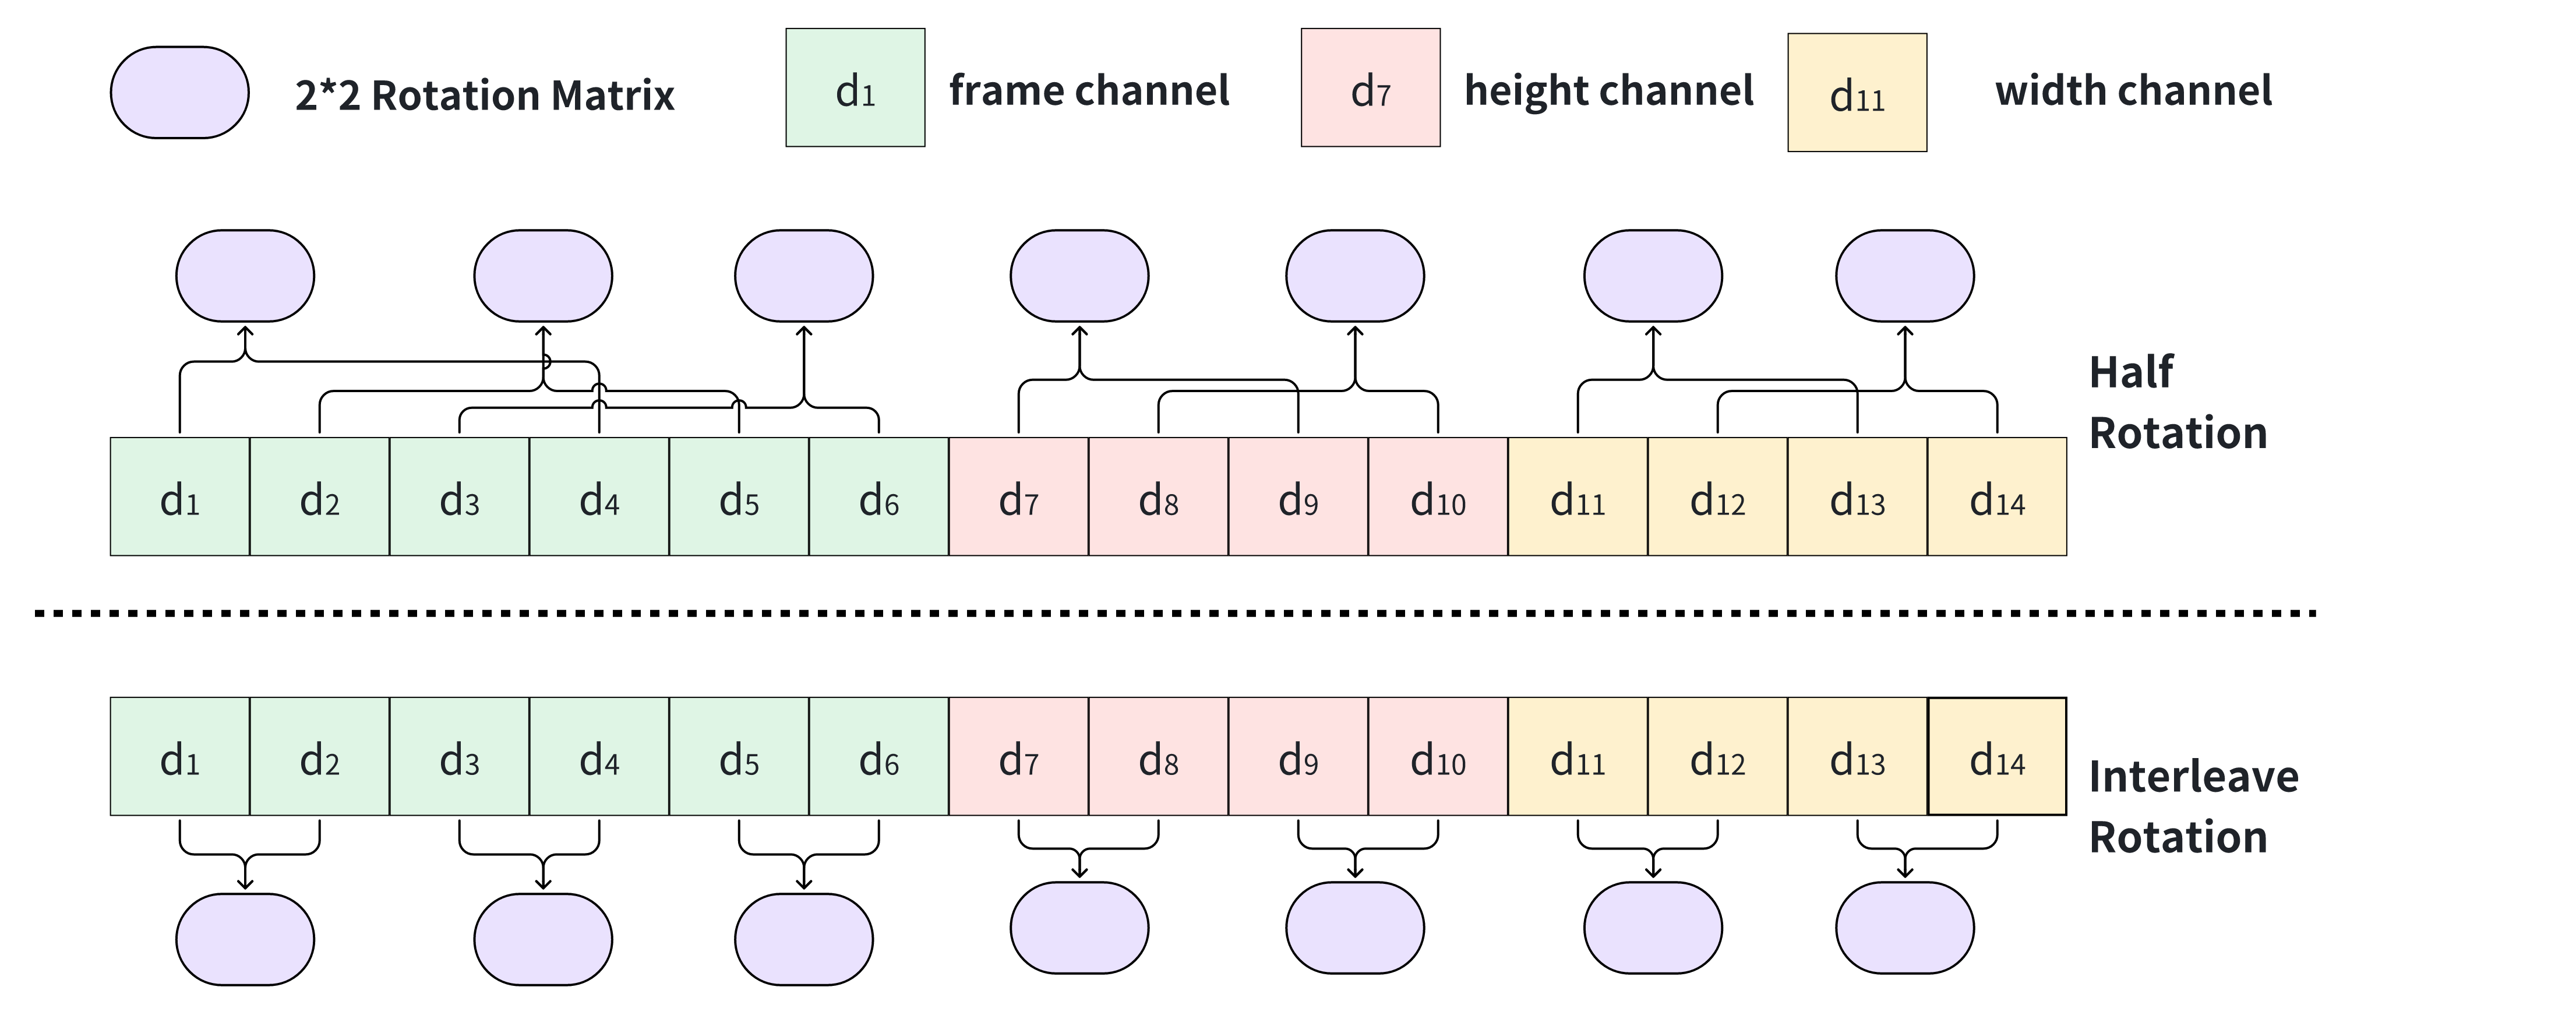
\includegraphics[width=1\linewidth]{eccv2026/samll_2/rotation.png}
    \caption{\textbf{Rotation strategies for $\mathbf{Q}$ and $\mathbf{K}$}. Interleaved Rotation groups adjacent dimensions into $2 \times 2$ orthogonal blocks, while Half Rotation pairs each dimension with its counterpart in the other half-segment.}
    \label{fig:rotation_strategies}
\end{figure*}



To integrate with RoPE, we design \textit{Interleaved Rotation}. We define a block-diagonal orthogonal matrix $\mathbf{R}$, where each $2 \times 2$ block acts on adjacent channel pairs $(d_{2i}, d_{2i+1})$ for $i \in \{1, \dots, D/2\}$. This transformation redistributes incoherence, yielding a more uniform outlier profile across the feature dimensions of $\mathbf{Q}$ and $\mathbf{K}$.

The core advantage of this design is its \textbf{operator mergeability}. Since both the rotary matrix $\mathbf{M}$ and our rotation $\mathbf{R}$ consist of $2 \times 2$ orthogonal blocks, their product $\mathbf{M}' = \mathbf{R}\mathbf{M}$ (or $\mathbf{M}\mathbf{R}$) preserves the block-diagonal structure. Consequently, the operations can be fused:
\begin{equation}
    \text{RoPE}(\mathbf{Q})\mathbf{R} = \mathbf{Q}(\mathbf{M}\mathbf{R}), \quad \text{RoPE}(\mathbf{K})\mathbf{R} = \mathbf{K}(\mathbf{M}\mathbf{R}).
\end{equation}
Because $\mathbf{M}\mathbf{R}$ maintains the same sparsity pattern as $\mathbf{M}$, it remains fully compatible with standard element-wise RoPE kernels. By pre-fusing $\mathbf{R}$ into the RoPE weights, we achieve outlier redistribution with \textbf{zero inference overhead}, providing a "free" improvement to quantization precision.


\subsubsection{Half Rotation}
\label{sssec:half_rotation}

Since outliers predominantly occupy one half of each segment, we introduce \textbf{Half Rotation}---a low-cost strategy that couples dimensions $d^j_{i}$ and $d^j_{i+D_j/2}$ for $i \in \{1, \dots, D_j/2\}$. Here, $d^j_{i}$ represents the $i$-th dimension of segment $j \in \{f, h, w\}$.

We define a block-diagonal permutation matrix $\mathbf{\Pi} = \mathrm{diag}(\mathbf{\Pi}^f, \mathbf{\Pi}^h, \mathbf{\Pi}^w)$, where each $\mathbf{\Pi}^j$ reorders the dimensions of segment $j$ such that dimensions separated by $D_j/2$ are moved to adjacent positions. The rotation matrix $\mathbf{R}$ is similarly structured as $\mathbf{R} = \mathrm{diag}(\mathbf{R}^f, \mathbf{R}^h, \mathbf{R}^w)$, where each $\mathbf{R}^j$ consists of $D_j/2$ orthogonal blocks $\mathbf{R}^j_k \in \mathrm{O}(2)$.

The final rotated query matrix is obtained via segment-wise transformation and concatenation:
\begin{equation}
    \mathbf{Q}\mathbf{\Pi}\mathbf{R} = \left[ \mathbf{Q}_f \mathbf{\Pi}^f \mathbf{R}^f, \mathbf{Q}_h \mathbf{\Pi}^h \mathbf{R}^h, \mathbf{Q}_w \mathbf{\Pi}^w \mathbf{R}^w \right].
\end{equation}

For each segment, the operation $\mathbf{Q}_j(\mathbf{\Pi}^j \mathbf{R}^j)$ exploits the inherent sparsity of the combined permutation-rotation matrix. Consequently, this matrix multiplication can be transformed into a highly efficient element-wise operation, analogous to the optimized implementation of RoPE. Through Half Rotation, incoherence is effectively equalized across the entire segment while maintaining high computational efficiency.

Fig.~\ref{fig:rotation_strategies} summarizes the two proposed RoPE-aware rotation strategies. Interleaved Rotation groups adjacent channel dimensions and can be merged into RoPE, while Half Rotation pairs dimensions across the two half-segments to equalize RoPE-induced outliers with negligible overhead.



\subsubsection{Learnable Rotation (Preliminary)}
\label{sssec:learnable_rotation}

As a preliminary investigation, we also explore making the rotation \textbf{learnable}. Let $\mathbf{Y} = \mathbf{Q}^{(s)}(\mathbf{K}^{(s)})^\top$ denote the full-precision attention score matrix computed from the smoothed query and key matrices. We learn the rotation matrix $\mathbf{R}$ by minimizing the following calibration objective with gradient-based optimization:
\begin{align}
\mathbf{R}^{\star}
&=
\arg\min_{\{\mathbf{R}_i\}}
\left\|
\mathbf{Y}
-
\mathcal{Q}\!\left(\mathbf{Q}^{(s)}\mathbf{R}\right)
\mathcal{Q}\!\left((\mathbf{K}^{(s)}\mathbf{R})^\top\right)
\right\|_F^2,
\label{eq:learnable_rotation_obj}
\\
&\quad\text{s.t.}\quad
\mathbf{R}_i \in \mathrm{O}(2), \quad i=1,\dots,D/2 .
\end{align}
Here, $\mathbf{Q}^{(s)}$ and $\mathbf{K}^{(s)}$ are the smoothed matrices, and $\mathcal{Q}(\cdot)$ denotes the quantization function. As shown in \cref{sssec:orthogonal_property}, this orthogonality constraint is essential---without it, the rotation degrades attention output quality, confirming that LLM-style unconstrained rotations~\cite{liu2025spinquant,sun2025flatquant} do not transfer to 
mixed-precision INT4 attention in 3D-RoPE video DiTs.
% video diffusion settings.
This experiment serves primarily to validate the orthogonality requirement; a thorough calibration study is left to future work (see \cref{sec:experiments}).


\subsection{Range-optimized $\mathbf{P}$ Quantization}

In the FlashAttention framework \cite{dao2022flashattention,dao2024flashattention,shah2024flashattention}, the attention scores are computed block-wise. Let $\mathbf{S}_{i,j} = \mathbf{Q}_i \mathbf{K}_j^\top / \sqrt{D}$ denote the pre-softmax attention scores for a given block. To maintain numerical stability during the online softmax process, a running row maximum $m_{i,j} = \max(m_{i,j-1}, \text{rowmax}(\mathbf{S}_{i,j}))$ is tracked, and the local attention probabilities are defined as $\mathbf{P}_{i,j} = \exp(\mathbf{S}_{i,j} - m_{i,j})$.

\subsubsection{Affine Range Expansion}

Standard quantization practices typically normalize the attention probabilities by their maximum value to fit the target bit-width. For $\text{INT4}$ symmetric quantization, the mapping is:
\begin{equation}
    \tilde{\mathbf{P}}_{i,j}^{\text{sym}} = \left\lfloor \frac{\mathbf{P}_{i,j}}{\max(\mathbf{P}_{i,j})} \times 7 \right\rceil \in (0, 7].
\end{equation}
This approach, however, leaves the negative representative space of $\text{INT4}$ ($[-8, 0)$) entirely unused, effectively wasting half of the available quantization levels and leading to significant precision loss.

To maximize the utilization of the 4-bit dynamic range, we propose a mapping with a fixed scale of $15$ and a zero-point of $-8$. This affine transformation projects the normalized probabilities onto the full $\text{INT4}$ interval $[-8, 7]$:
\begin{equation}
    \tilde{\mathbf{P}}_{i,j} = \left( \frac{\mathbf{P}_{i,j}}{\max(\mathbf{P}_{i,j})} \times 15 \right) - 8 \in (-8, 7].
\end{equation}
By expanding the representation from 8 levels ($0$ to $7$) to 16 levels ($-8$ to $7$), we effectively double the quantization resolution, significantly reducing the rounding error.




\subsection{Hadamard Transformation for the Value Matrix}
\label{ssec:hadamard_v}

To mitigate the impact of outliers within the Value matrix $\mathbf{V}$, we employ an orthogonal rotation transformation using a $D \times D$ Hadamard matrix $\mathbf{H}$, where $D = 2^n$ ($n \in \mathbb{Z}^+$). The $2 \times 2$ Hadamard matrix is defined in \cref{eq:H_2}. Hadamard matrices are constructed recursively via the Kronecker product:
\begin{equation}
\mathbf{H}_{2^{n}} = \mathbf{H}_{2} \otimes \mathbf{H}_{2^{n-1}}.
\end{equation}


The Hadamard rotation can be mathematically absorbed into the value projection $\mathbf{W}_v$ and the output projection $\mathbf{W}_o$. Given the value projection $\mathbf{V} = \mathbf{X}\mathbf{W}_v$, the standard attention output is:


\begin{align}
\mathbf{O} &= \text{Softmax}\left(\frac{\mathbf{Q}\mathbf{K}^\top}{\sqrt{d_k}}\right) \mathbf{V} \mathbf{W}_o \nonumber \\
 &= \text{Softmax}\left(\frac{\mathbf{Q}\mathbf{K}^\top}{\sqrt{d_k}}\right) \mathbf{X} (\mathbf{W}_v \mathbf{H}) (\mathbf{H}^\top \mathbf{W}_o).
\end{align}

\newpage


We can merge the Hadamard transform into the weights as $\widetilde{\mathbf{W}}_v=\mathbf{W}_v\mathbf{H}$ and $\widetilde{\mathbf{W}}_o=\mathbf{H}^{\top}\mathbf{W}_o$, respectively. Since these modified weights are computed offline during the preprocessing stage, the Hadamard transformation for $\mathbf{V}$ is achieved with \textbf{zero additional computational overhead} during inference.



